%%%%%%%%%%%%%%%%%%%%%%%%%%%%%%%%%%%%%%%%%
% Sullivan Business Report
% LaTeX Template
% Version 1.0 (May 5, 2022)
%
% This template originates from:
% https://www.LaTeXTemplates.com
%
% Author:
% Vel (vel@latextemplates.com)
%
% License:
% CC BY-NC-SA 4.0 (https://creativecommons.org/licenses/by-nc-sa/4.0/)
%
%%%%%%%%%%%%%%%%%%%%%%%%%%%%%%%%%%%%%%%%%


%----------------------------------------------------------------------------------------
%	CLASS, PACKAGES AND OTHER DOCUMENT CONFIGURATIONS
%----------------------------------------------------------------------------------------

\documentclass[
    a4paper, % Paper size, use either a4paper or letterpaper
	12pt, % Default font size, the template is designed to look good at 12pt so it's best not to change this
	%unnumberedsections, % Uncomment for no section numbering
    ]{CSSullivanBusinessReport}
    
    \addbibresource{sample.bib} % BibLaTeX bibliography file

%----------------------------------------------------------------------------------------
%	REPORT INFORMATION
%----------------------------------------------------------------------------------------

\reporttitle{CPE 233 Hardware Assignment 6} % The report title is to appear on the title page and page headers, do not create manual new lines here as this will carry over to page headers

\reportsubtitle{Assembling the MCU} % Report subtitle, include new lines if needed

\reportauthors{Report by:\\\smallskip Ethan Vosburg (evosburg@calpoly.edu)} % Report authors/group/department, include new lines if needed

\reportdate{\today} % Report date, include new lines for additional information if needed

\rightheadercontent{
\includegraphics[width=3cm]{creodocs_logo.pdf}} % The content in the right header, you may want to add your own company logo or use your company/department name or leave this command empty for no right header content

%----------------------------------------------------------------------------------------

\begin{document}

%----------------------------------------------------------------------------------------
%	TITLE PAGE
%----------------------------------------------------------------------------------------

\thispagestyle{empty} % Suppress headers and footers on this page

\begin{fullwidth} % Use the whole page width
	\vspace*{-0.075\textheight} % Pull logo into the top margin
	
	\hfill
\includegraphics[width=5cm]{creodocs_logo.pdf} % Company logo

	\vspace{0.15\textheight} % Vertical whitespace

	\parbox{0.9\fulltextwidth}{\fontsize{50pt}{52pt}\selectfont\raggedright\textbf{\reporttitle}\par} % Report title, intentionally at less than full width for nice wrapping. Adjust the width of the \parbox and the font size as needed for your title to look good.
	
	\vspace{0.03\textheight} % Vertical whitespace
	
	{\LARGE\textit{\textbf{\reportsubtitle}}\par} % Subtitle
	
	\vfill % Vertical whitespace
	
	{\Large\reportauthors\par} % Report authors, group or department
	
	\vfill\vfill\vfill % Vertical whitespace
	
	{\large\reportdate\par} % Report date
\end{fullwidth}

\newpage

%----------------------------------------------------------------------------------------
%	DISCLAIMER/COPYRIGHT PAGE
%----------------------------------------------------------------------------------------

% \thispagestyle{empty} % Suppress headers and footers on this page

% \begin{twothirdswidth} % Content in this environment to be at two-thirds of the whole page width
% 	\footnotesize % Reduce font size
	
% 	\subsection*{Disclaimer}

% 	Lorem ipsum dolor sit amet, consectetur adipiscing elit. Praesent porttitor arcu luctus, imperdiet urna iaculis, mattis eros. Pellentesque iaculis odio vel nisl ullamcorper, nec faucibus ipsum molestie. Sed dictum nisl non aliquet porttitor. Etiam vulputate arcu dignissim, finibus sem et, viverra nisl. Aenean luctus congue massa, ut laoreet metus ornare in. Nunc fermentum nisi imperdiet lectus tincidunt vestibulum at ac elit.
	
% 	\subsection*{Copyright}
	
% 	\textcopyright~[Year] [Company] 
	
% 	Copyright notice text\ldots In hac habitasse platea dictumst. Curabitur mattis elit sit amet justo luctus vestibulum. In hac habitasse platea dictumst. Pellentesque lobortis justo enim, a condimentum massa tempor eu. Ut quis nulla a quam pretium eleifend nec eu nisl. Nam cursus porttitor eros, sed luctus ligula convallis quis.
	
% 	\subsection*{Contact}
	
% 	Address Line 1\\
% 	Address Line 2\\
% 	Address Line 3
	
% 	Business Number 123456
	
% 	Contact: name@company.com
	
% 	\vfill % Push the following down to the bottom of the page
	
% 	\subsubsection*{Changelog}
	
% 	\scriptsize % Reduce font size further
	
% 	\begin{tabular}{@{} L{0.05\linewidth} L{0.15\linewidth} L{0.6\linewidth} @{}} % Column widths specified here, change as needed for your content
% 		\toprule
% 		v1.0 & 20XX-02-05 & Lorem ipsum dolor sit amet, consectetur adipiscing elit. Praesent porttitor arcu luctus, imperdiet urna iaculis, mattis eros.\\
% 		v1.1 & 20XX-02-27 & Pellentesque iaculis odio vel nisl ullamcorper, nec faucibus ipsum molestie.\\
% 		v1.2 & 20XX-03-15 & Sed dictum nisl non aliquet porttitor.\\
% 		\bottomrule
% 	\end{tabular}
% \end{twothirdswidth}

% \newpage

%----------------------------------------------------------------------------------------
%	TABLE OF CONTENTS
%----------------------------------------------------------------------------------------
\bigskip
\begin{twothirdswidth} % Content in this environment to be at two-thirds of the whole page width
	\tableofcontents % Output the table of contents, automatically generated from the section commands used in the document
\end{twothirdswidth}

\newpage
%----------------------------------------------------------------------------------------
%	SECTIONS
%----------------------------------------------------------------------------------------
\begin{fullwidth} % Use the whole page width

\section{Project Description} % Top level section

In this project the central component of a functional microcontroller (MCU) is constructed by integrating various OTTER modules developed in previous assignments. While the resulting MCU will not represent the complete OTTER system, it will serve as a foundational unit for future expansions. This assignment will build the foundation for the rest of the hardware assignments as the OTTER starts to take shape and we can begin to implement it on the Basys3 board.

\subsection{Control Unit Decoder}
The Control Unit Decoder is a combinational logic component responsible for generating control signals based on the current instruction. Unlike the Control Unit FSM, the signals generated by the decoder are less time-sensitive, allowing for a simpler, combinational design. The decoder takes the instruction opcode as input and outputs control signals to various components of the MCU, such as the ALU, registers, and memory units. The primary function of the decoder is to interpret the instruction and set the appropriate control signals to execute the operation specified by the instruction.

% \begin{enumerate}
%     \item Input: Receives the opcode part of the instruction.
%     \item Processing: Decodes the opcode to determine the operation to be performed.
%     \item Output: Generates control signals based on the decoded operation. These signals are sent to the relevant components of the MCU to carry out the instruction.
% \end{enumerate}
\subsection{Control Unit FSM}
The Control Unit FSM is responsible for controlling the timing-critical aspects of the MCU's operation. It operates in three main states: FETCH, EXEC, and WRITEBACK. The FSM ensures that instructions are fetched, executed, and the results are written back in a controlled manner, particularly for operations involving memory access.

\subsection{OTTER MCU}
The OTTER MCU is a microcontroller unit composed of various modules, including the Control Unit (with its FSM and Decoder), ALU, registers, and memory units. It is designed to execute a set of instructions, manipulating data and performing operations as specified by the program.



\section{Structural Design} % Second level section

\subsection{OTTER MCU} % Third level section

\begin{figure}[H]
    \centering
    \captionsetup{style=widetable}
    \makebox[.80\pdfpagewidth]{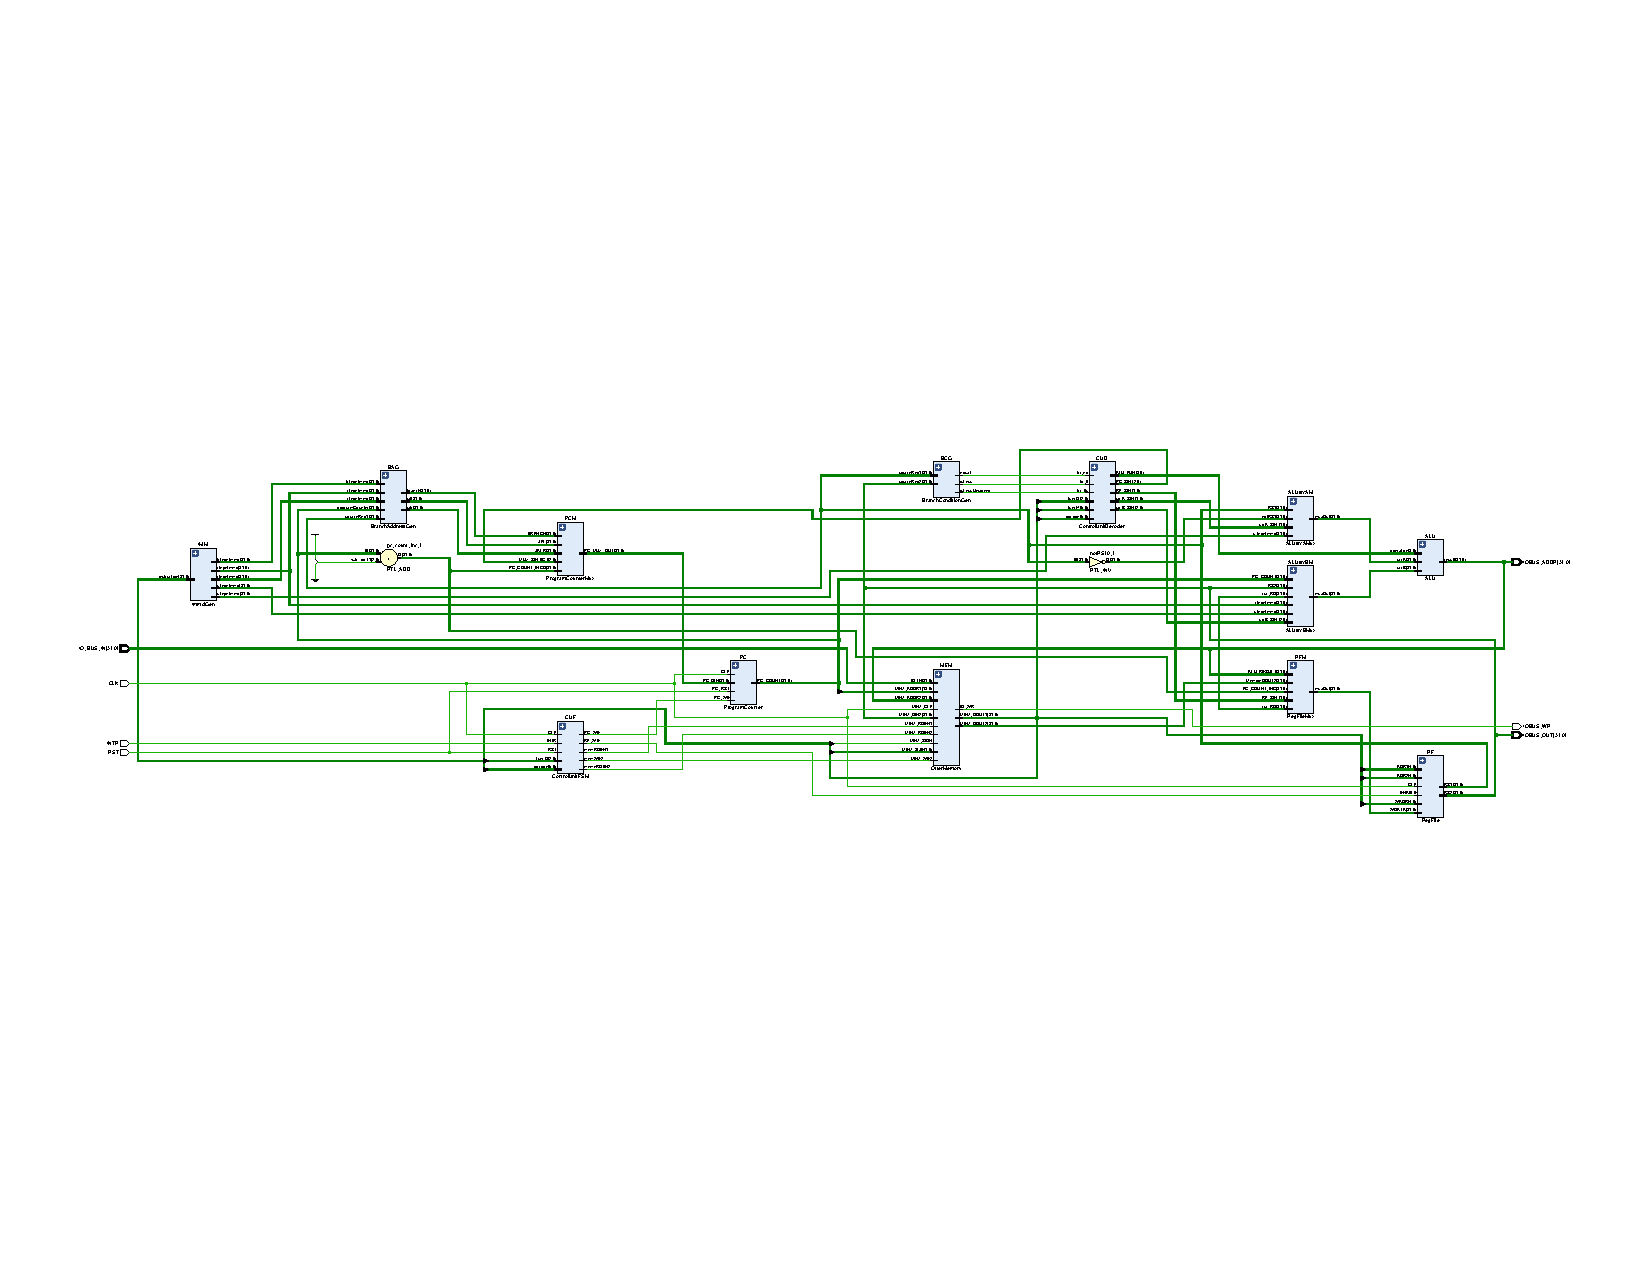
\includegraphics[width=.90\pdfpagewidth]{Figures/MCUschematic.pdf}}
    \caption{OTTER MCU Eleborated Design}
    \label{fig:MCUschematic}
\end{figure}

\section{Synthesis Warnings} % Second level section

\subsection{MCU Synthesis Warnings} % Third level section
\begin{figure}[H]
    \captionsetup{style=widetable}
    \makebox[.80\pdfpagewidth]{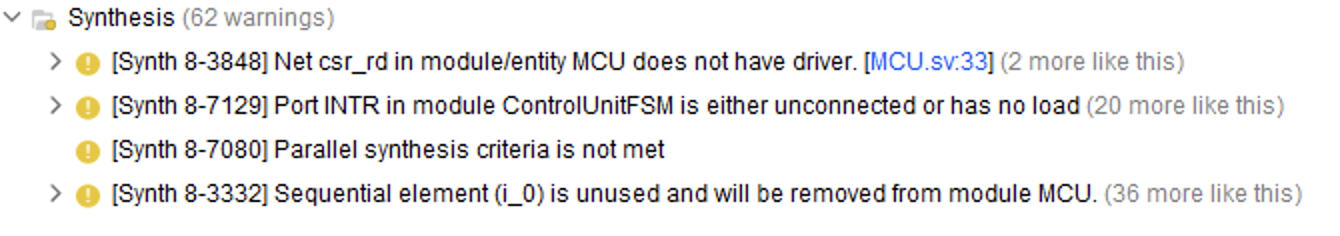
\includegraphics[width=.75\pdfpagewidth]{Figures/Synthesis Warnings.png}}
    \caption{Synthesis Warnings for MCU}
    \label{fig:MCUWarnings}
\end{figure}

The warnings referenced in Figure \ref{fig:MCUWarnings} are not important as there is hardware that will still need to be implemented in future assignments. This means there are various wires that do not have a driver or that do not lead to a defined location. This is fine and in this case does not prevent the design from working. Vivado is simply letting you know that these lines will not be implemented in to the design at this point.

\section{Verification} % Second level section

\begin{figure}[H]
    \captionsetup{style=widetable}
    \makebox[.80\pdfpagewidth]{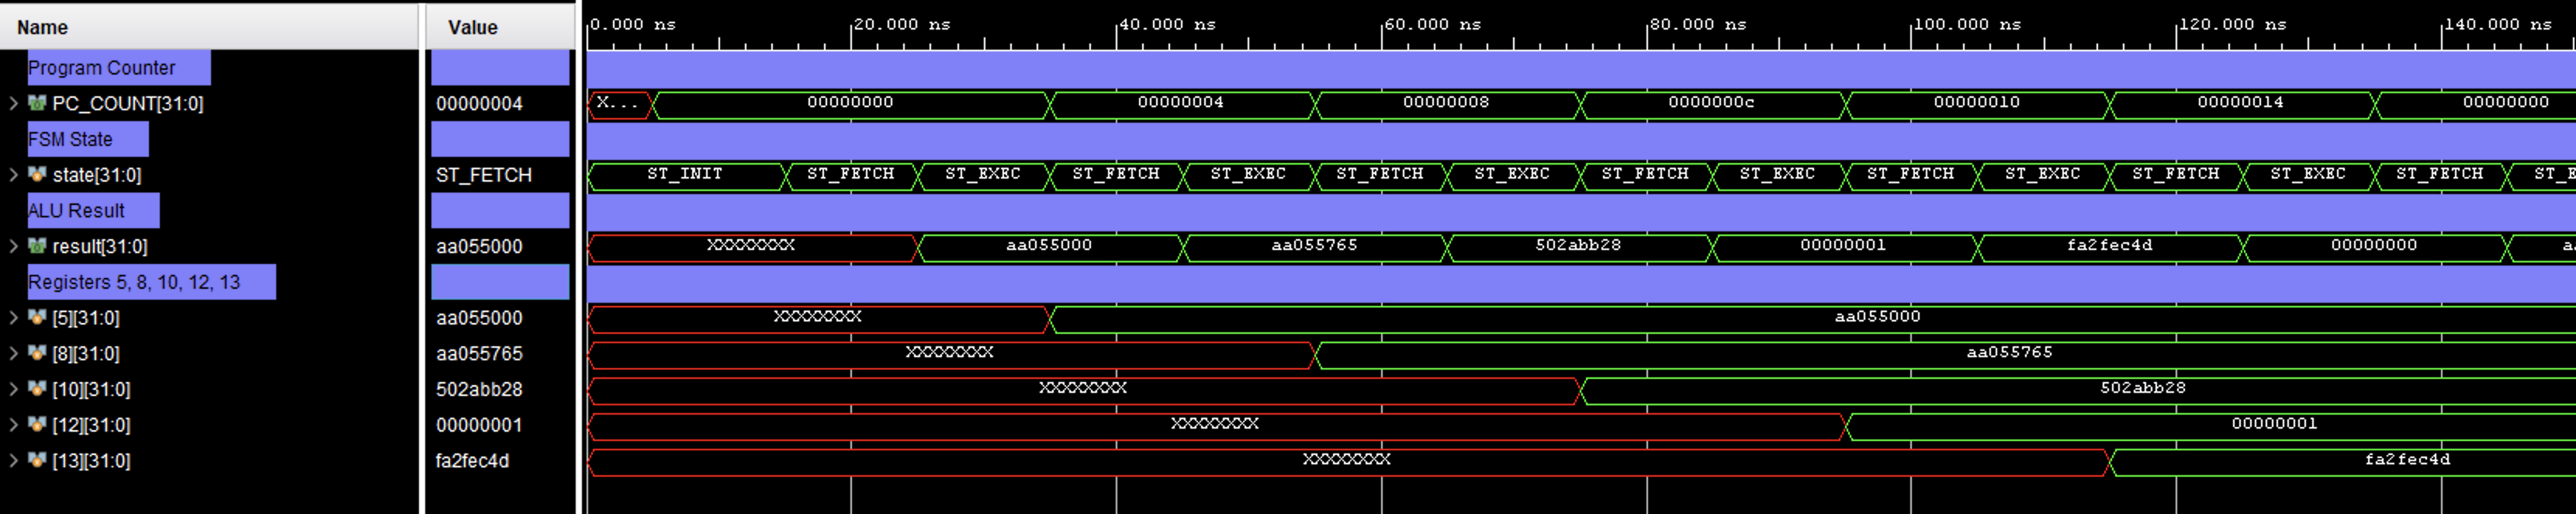
\includegraphics[width=.75\pdfpagewidth]{Figures/OTTER MCU Simulation.png}}
    \caption{OTTER MCU Verification}
    \label{fig:otterVerification}
\end{figure}

\begin{figure}[H]
    \captionsetup{style=widetable}
    \makebox[.80\pdfpagewidth]{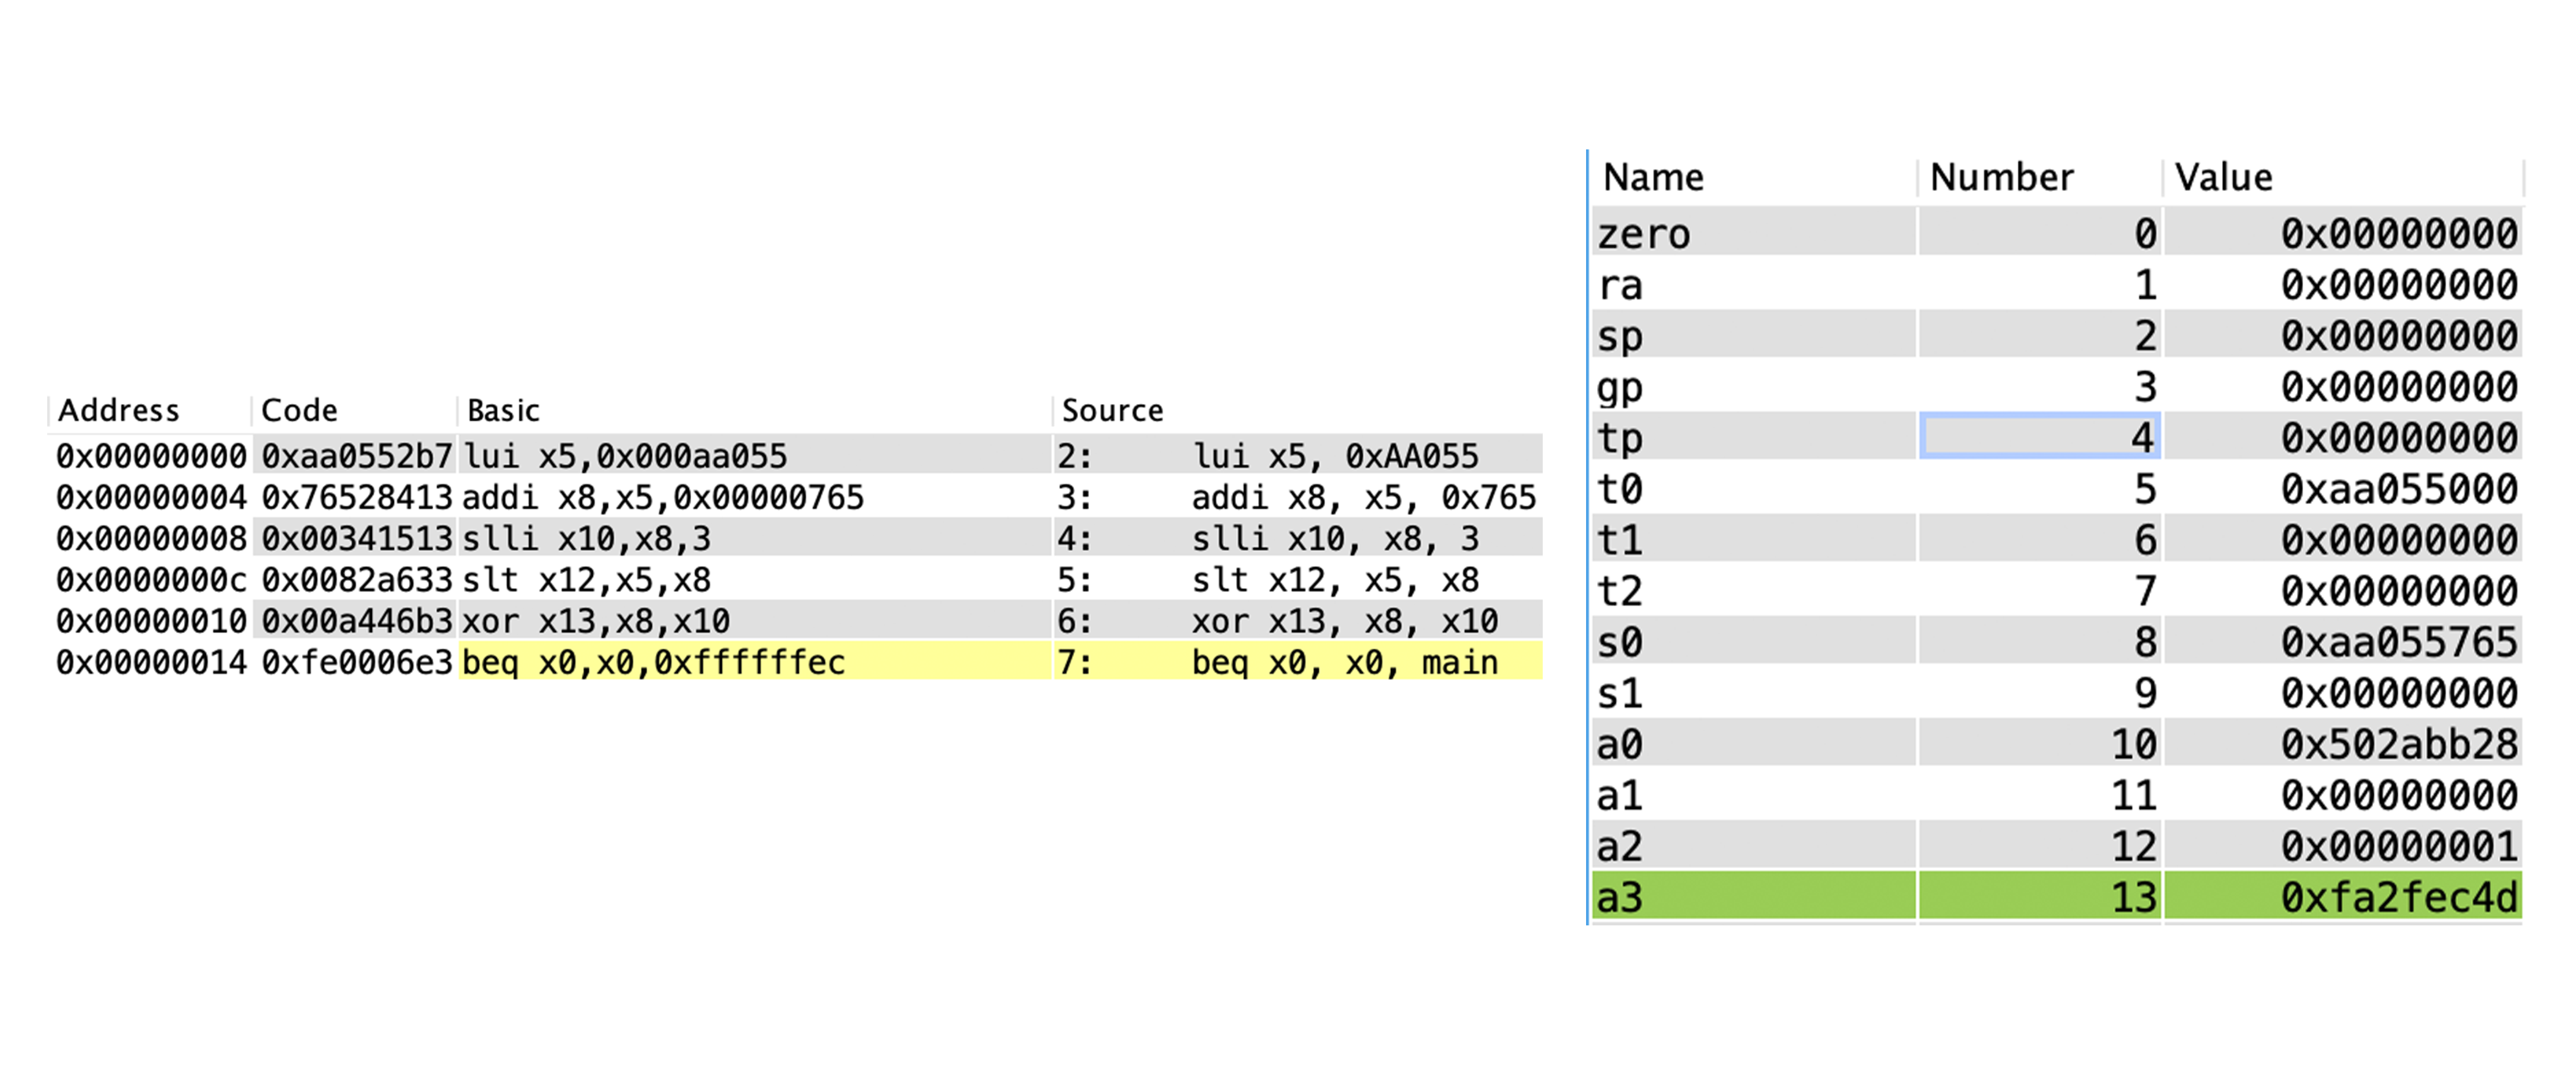
\includegraphics[width=.75\pdfpagewidth]{Figures/OTTER MCU RARS.png}}
    \caption{OTTER MCU RARS Simulation}
    \label{fig:rarsVerification}
\end{figure}

Looking at the simulation we have the outputs that we would expect referencing figure \ref{fig:rarsVerification} you can compare the hex values for the registers and see that they all match up. They registers have an undefined value before they are written to which is expected. Also There is a longer INIT state becuase of the reset command in the beginning of the file.

\newpage
\section{Source Code}
\captionsetup{style=widetable}
\subsection{Branch Address Generator Source Code} % Third level section

\lstinputlisting[language=Verilog, caption=Control Unit FSM]{/Users/ethanvosburg/Documents/git/CPE-233-Otter/HW6-MCU/MCU/MCU.srcs/sources_1/new/ControlUnitFSM.sv}
\newpage


\lstinputlisting[language=Verilog, caption=Control Unit Decoder]{/Users/ethanvosburg/Documents/git/CPE-233-Otter/HW6-MCU/MCU/MCU.srcs/sources_1/new/ControlUnitDecoder.sv}

\newpage
\lstinputlisting[language=Verilog, caption=Master MCU Linking all Modules Together]{/Users/ethanvosburg/Documents/git/CPE-233-Otter/HW6-MCU/MCU/MCU.srcs/sources_1/new/MCU.sv}




\section{Conclusion} % Second level section
\hypersetup{urlcolor=blue} 
In this project, the MCU was sussesfully constructed and tested with a limited set of code. The ground work for future hardware compnents was made tested to be working. This is the culmination of all the modules that have been made to this point and represents the first time that the compnents have all worked together. From here more moduels can be added to add more funcitonality.
All code for this assignment can be found \href{https://github.com/EthanV1920/CPE-233-Otter/tree/main}{here}.


\end{fullwidth}

\end{document}